\section{Experimental Evaluation}\label{sec:evaluation}

\subsection{Evaluation Design and Testbed}
% Removed: The evaluation combines (i)~a functional validation campaign over the full enrollment-to-deployment path and (ii)~a sustainability-oriented measurement pass on the same test bed.
{\color{red}The evaluation combines (i)~a functional validation campaign over the full enrollment-to-deployment path and (ii)~a sustainability-oriented measurement pass on the same testbed.} The functional study asks whether cloud intent, gateway mediation, and embedded WASM execution produce mutually consistent evidence under repeatable conditions. The sustainability pass quantifies southbound wire sizes, edge firmware footprint, and Kubernetes pod resource use. 
%Neither pass claims measured joules or carbon reductions; they establish baselines relevant to green-experimentation follow-up.

Experiments run on a single-node K3s cluster with API server, gateway, application controller, and CRDs active. The southbound endpoint is a Renode-emulated STM32F746 running Zephyr firmware with WAMR and connects over TAP-based networking with DNAT to the gateway TLS port. Table~\ref{tab:testbed} summarizes the host and software stack.

\begin{table}[pos=t]
\centering
\caption{Experimental testbed and software configuration.}%
\label{tab:testbed}
\footnotesize
\setlength{\tabcolsep}{3pt}
\begin{tabular}{p{0.30\linewidth} p{0.62\linewidth}}
\toprule
\textbf{Item} & \textbf{Configuration} \\
\midrule
Host OS & Ubuntu 24.04 LTS (kernel 6.8.0), x86\_64 KVM guest \\
Host resources & 32 vCPUs, 62~GiB RAM, 293~GiB SSD \\
Orchestrator & K3s v1.35.4+k3s1, single control-plane node \\
Southbound emulation & Renode \texttt{antmicro/renode:nightly}, board \texttt{Stm32F746gDisco} \\
Firmware stack & Zephyr RTOS 3.5.0, WAMR 2.4.1, minimal WASM test module (33~B) \\
Device networking & Bridge \texttt{wasmbr0} at 192.168.1.1/24, one TAP per device, DHCP, DNAT to the gateway pod's TLS port \\
\bottomrule
\end{tabular}
\end{table}

% Removed: After one warm-up run, the campaign executes $n{=}100$ independent trials.
{\color{red}After one warm-up run, the campaign executes $n{=}100$ repeated enrollment-to-deployment trials started from a known logical state.} Each trial performs enrollment verification, heartbeat supervision, and deployment of the minimal WASM module to the same emulated device. A trial is \emph{transactionally} successful only if all three stages succeed and deployment evidence is consistent across the gateway runtime view and the Application CRD (\texttt{phase=Running}, device connected, fresh heartbeat). Continuous latencies use monotonic client-side timers; we report mean, standard deviation, median, p95, p99, IQR, CV, and 95\% CI of the mean ($\bar{x} \pm t_{0.975,n-1}\,s/\sqrt{n}$, with $t_{0.975,99}{=}1.984$). For binary outcomes we use Wilson score intervals; with 100/100 successes the 95\% lower bound is 96.3\%.

\revC{Two caveats govern how these summaries should be read. First, consecutive trials share the same host, the same warmed page cache, the same already-compiled runtime and the same long-lived control-plane processes, so they are repetitions rather than independent draws: we report the $t$-based intervals as descriptive dispersion summaries of this campaign, not as inferential statements about a wider population of deployments or about heterogeneous devices, gateways and physical networks, and we check the assumption directly on the trial series (Figure~\ref{fig:latency-trial-scatter}). The end-to-end series shows no accumulation and no drift: the lag-1 autocorrelation is $-0.09$, the Spearman rank correlation between latency and trial index is $-0.14$ ($t{=}{-}1.42$, not significant at $n{=}100$), and the first and second halves of the campaign have means of 1212.1~ms and 1159.5~ms with standard deviations of 184.7~ms and 142.2~ms. The campaign is thus stationary after the discarded warm-up run. Second, the campaign induces no faults: no packet loss, no gateway restart, no key mismatch, no contention from co-located tenants. Under those conditions, 100/100 confirms that the cross-layer evidence-convergence criterion of Table~\ref{tab:trial-semantics} holds whenever the mechanism is exercised without induced failure, and the Wilson lower bound of 96.3\% is the arithmetic consequence of that fault-free protocol rather than an availability figure for a production fleet.}

\begingroup
\color{red}
\subsection{Trial Procedure and Evidence Semantics}
The harness starts from a known logical state, observes the device enrollment path, waits for heartbeat evidence to become visible through the gateway, creates or updates the Application intent, and then checks whether the gateway runtime view and Kubernetes status converge to the same deployment outcome.

The measurement record separates four kinds of evidence. First, protocol evidence comes from enrollment, heartbeat, and deployment records exchanged over the TLS/CBOR channel. Second, gateway evidence comes from the runtime association between a device identifier and an active session. Third, Kubernetes evidence comes from Device and Application status fields after reconciliation. Fourth, timing evidence comes from the client-side harness using monotonic timestamps around the evaluated stages. A trial succeeds only when these evidence sources agree before the configured timeout. This convention reduces the risk of reporting success from a single eventually consistent field or from a transport acknowledgment that never becomes durable control-plane state.

Latency measurements follow the same separation. Enrollment latency measures the interval needed to complete the identity-binding path and expose the enrolled device to the control plane. Deployment latency measures the path from declared Application intent to reported execution outcome. End-to-end latency is the sum of enrollment and deployment for the evaluated transaction. Heartbeat observability is reported separately because it measures how quickly the harness can observe a fresh heartbeat after it is available through the gateway; it is not the firmware heartbeat period and should not be interpreted as a liveness interval.

\begin{table}[pos=t]
\centering
\caption{Trial-level success and failure interpretation.}
\label{tab:trial-semantics}
\footnotesize
\setlength{\tabcolsep}{3pt}
\begin{tabular}{p{0.28\linewidth} p{0.62\linewidth}}
\toprule
\textbf{Condition} & \textbf{Trial interpretation} \\
\midrule
Enrollment accepted but identity not matched to the expected Device resource & Failure, because a protected channel alone is not a platform-level attachment. \\
Heartbeat received by the gateway but not reflected as fresh liveness evidence & Failure for the transaction, because the control plane cannot rely on the observation. \\
Deploy command acknowledged but Application status does not converge & Failure, because command dispatch is not equivalent to verifiable execution. \\
Application status reports success while gateway or Device evidence is inconsistent & Failure, because cross-layer evidence does not agree. \\
Enrollment, heartbeat freshness, gateway association, and Application outcome agree & Transactional success. \\
\bottomrule
\end{tabular}
\end{table}
\endgroup


\subsection{Functional Validation Results}\label{sec:functional-results}
All 100 transactional trials completed successfully: enrollment, heartbeat supervision, deployment, and cross-layer evidence checks never failed. \revC{These trials exercise the enrollment path in which the Device resource reaches \texttt{phase}\,=\,\texttt{Connected} from gateway-observed session evidence, which is the path described in Section~\ref{sec:protocol} and the one the framework uses in normal operation.} %Removed (M8): Section~\ref{sec:energy-instrumentation} reports a separate, later instrumentation pass that provisions devices through the auxiliary HTTP registry endpoint instead, and the difference between the two is explained there.}
\revD{Section~\ref{sec:energy-instrumentation} reports a separate, later instrumentation
pass in which the same enrollment path is preceded by an explicit board registration
through the gateway HTTP endpoint, so that the resource creation cost falls inside the
measured window; the two passes exercise the same protocol stages and their latencies are
not compared.} %Removed (minore): Because {\color{red}every measured stage succeeded in all trials}, a per-stage success table would repeat identical Wilson bounds and is omitted; the meaningful variation lies in latency and its distribution.
\revD{Every measured stage succeeded in all trials, so the meaningful variation lies in latency and its distribution.}

Table~\ref{tab:quantitative-latency} reports the latency profile. Mean end-to-end latency {\color{red}(enrollment plus deployment; heartbeat observability reported separately)} is 1286.0~ms with 95\% CI [1226.4, 1345.6]~ms. %Removed (M9): Deployment carries a heavy upper tail (CV 0.43, maximum 3000.8~ms against a median of 574.1~ms) that the mean and the p95 both understate; it reproduces across independent campaigns on this testbed and is the dominant contribution to end-to-end variability.
\revD{Deployment carries a heavy upper tail (CV 0.43, maximum 3000.8~ms against a
median of 574.1~ms) that the mean and the p95 both understate. The tail is an artefact of
how the harness observes completion, not of the orchestration path: after issuing the
deployment the harness polls the Application resource on a fixed two-second cycle, so a
trial whose evidence becomes visible just after a poll is charged a full cycle. The raw
series is consistent with this. Seventy of the hundred trials fall in a narrow
487--598~ms band and twenty-eight more between 603 and 1112~ms; only two exceed that, the
largest at 3000.8~ms, a full polling cycle beyond the rest. The reported deployment latency is therefore
an upper bound that includes observation granularity, and the dispersion statistics of
this stage should be read as a property of the measurement procedure rather than of WASM
orchestration.}

\begin{table}[pos=t]
\centering
\caption{Latency profile ($n{=}100$ trials). All values in milliseconds.}%
\label{tab:quantitative-latency}
\footnotesize
\setlength{\tabcolsep}{2pt}
\resizebox{\columnwidth}{!}{%
\begin{tabular}{lrrrrrrr}
\toprule
\textbf{Stage} & \textbf{Mean} & \textbf{Median} & \textbf{p95} & \textbf{p99} & \textbf{IQR} & \textbf{CV} & \textbf{95\% CI of mean} \\
\midrule
Enrollment & 609.5 & 568.1 & 839.6 & 889.8 & 50.4 & 0.164 & [589.6, 629.4] \\
Heartbeat obs. & 4.08 & 4.01 & 4.97 & 5.29 & 0.53 & 0.114 & [3.99, 4.17] \\
Deployment & 676.5 & 574.1 & 1021.8 & 1145.2 & 228.4 & 0.428 & [619.1, 733.9] \\
End-to-end & 1286.0 & 1168.7 & 1661.5 & 1974.3 & 270.7 & 0.234 & [1226.4, 1345.6] \\
\bottomrule
\end{tabular}%
}
\end{table}

Figure~\ref{fig:latency-boxplot} compares stage latency distributions on a logarithmic scale. Heartbeat observability is two orders of magnitude faster than enrollment or deployment. %Removed (M9): Figure~\ref{fig:latency-cdf} shows that deployment contributes most of the tail mass: its p95 (1021.8~ms) and p99 (1145.2~ms) exceed enrollment's, so WASM orchestration, not TLS enrollment, dominates end-to-end variability (deployment CV\,=\,0.428 vs.\ enrollment CV\,=\,0.164).
\revD{Figure~\ref{fig:latency-cdf} shows that deployment contributes most of the tail
mass: its p95 (1021.8~ms) and p99 (1145.2~ms) exceed enrollment's, and its coefficient of
variation is correspondingly larger (0.428 against 0.164). Given the polling artefact
described above, this separates the two stages by how they are observed rather than by
their intrinsic cost: enrollment is timed on the protocol exchange itself, whereas
deployment is timed on the first poll that sees converged status.}

\begin{figure}[pos=t]
\centering
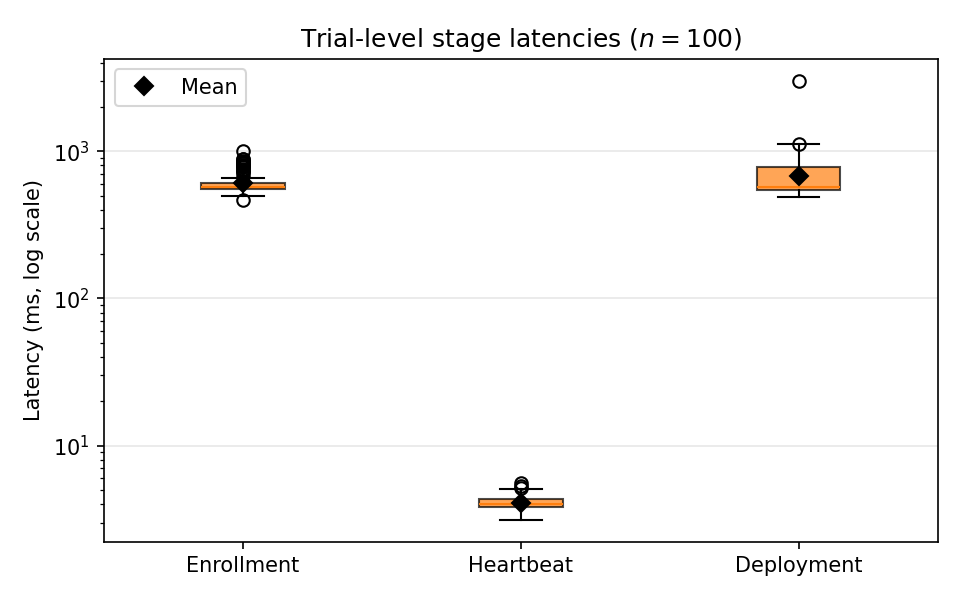
\includegraphics[width=\columnwidth]{figures/latency_boxplot.png}
\caption{Distribution of trial-level stage latencies ($n{=}100$, log scale). Diamonds indicate sample means.}%
\label{fig:latency-boxplot}
\end{figure}

\begin{figure}[pos=t]
\centering
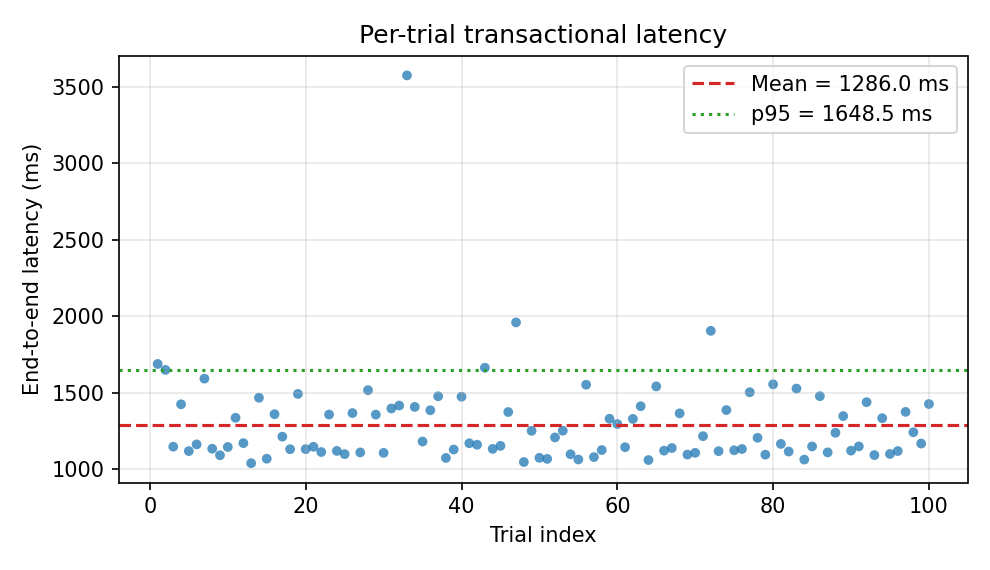
\includegraphics[width=\columnwidth]{figures/latency_trial_scatter.png}
\caption{\revC{End-to-end latency by trial index ($n{=}100$). The series is stationary after the discarded warm-up run; see Section~\ref{sec:evaluation} for the correlation statistics.}}%
\label{fig:latency-trial-scatter}
\end{figure}

\begin{figure}[pos=t]
\centering
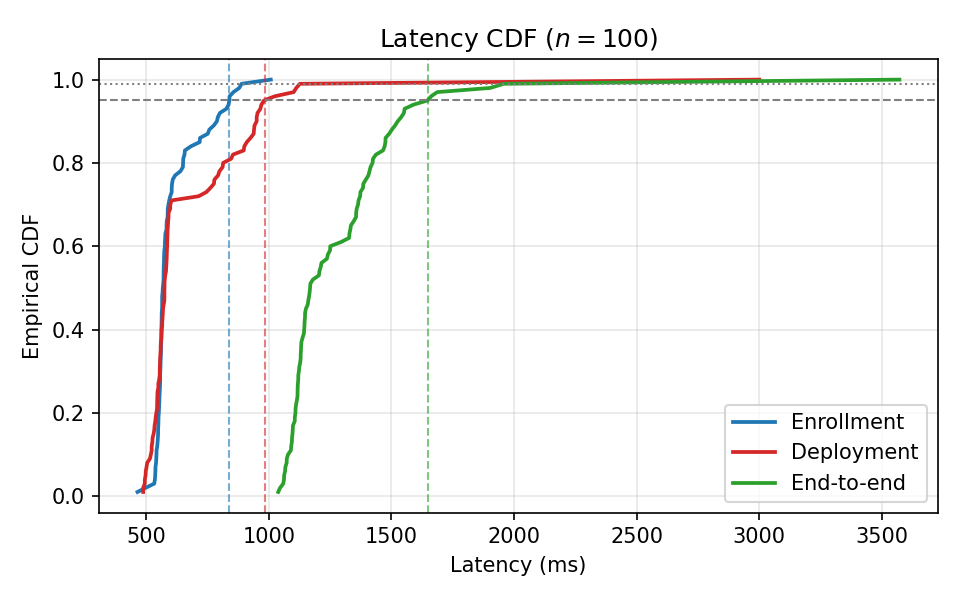
\includegraphics[width=\columnwidth]{figures/latency_cdf.png}
\caption{Empirical CDF of enrollment, deployment, and end-to-end latencies ($n{=}100$).}%
\label{fig:latency-cdf}
\end{figure}

\subsection{Sustainability-Oriented Metrics}\label{sec:sustainability-metrics}

\subsubsection{Southbound wire efficiency}
Application messages use a 4-byte big-endian length prefix followed by CBOR payloads. Figure~\ref{fig:wire-sizes} summarizes measured wire sizes for representative messages. Heartbeat request and acknowledgment are 6~B each; a complete enrollment round trip totals 87~B of application payload; a minimal deploy round trip (33~B WASM module) totals 90~B. % Removed: At the configured 25~s heartbeat period, steady-state control traffic is $12 \times (3600/25) = 1728$~B/h per device (${\approx}$1.69~KiB/h), excluding TLS record overhead.
{\color{red}At the configured 25~s heartbeat period, steady-state application-layer heartbeat traffic is $12 \times (3600/25) = 1728$~B/h per device (${\approx}$1.69~KiB/h), excluding TLS record overhead and lower-layer TCP/IP, Ethernet/TAP, and retransmission overhead.}

\revD{Because that exclusion spans more than an order of magnitude, we state the on-wire
cost analytically from the protocol constants, and mark it as an estimate rather than a
measurement. Under the evaluated TLS~1.2 AES-128-GCM cipher suite each record adds 5~B of
record header, an 8~B explicit nonce and a 16~B authentication tag, so a 6~B heartbeat
becomes a 35~B record, a 75~B IPv4 segment and a 93~B Ethernet frame. At a 25~s period the
delayed-acknowledgment timer expires between exchanges, so request and acknowledgment are
each acknowledged separately, giving roughly 300~B per heartbeat exchange and of order
40~KB/h per device: approximately $25\times$ the application-layer figure. Session
establishment is excluded from both numbers and is paid again on every reconnection, so a
device that re-handshakes frequently is dominated by that cost rather than by heartbeats.
A packet-capture measurement of steady-state and reconnection traffic, which would replace
this estimate, is left to future work.}

\begin{figure}[pos=t]
\centering
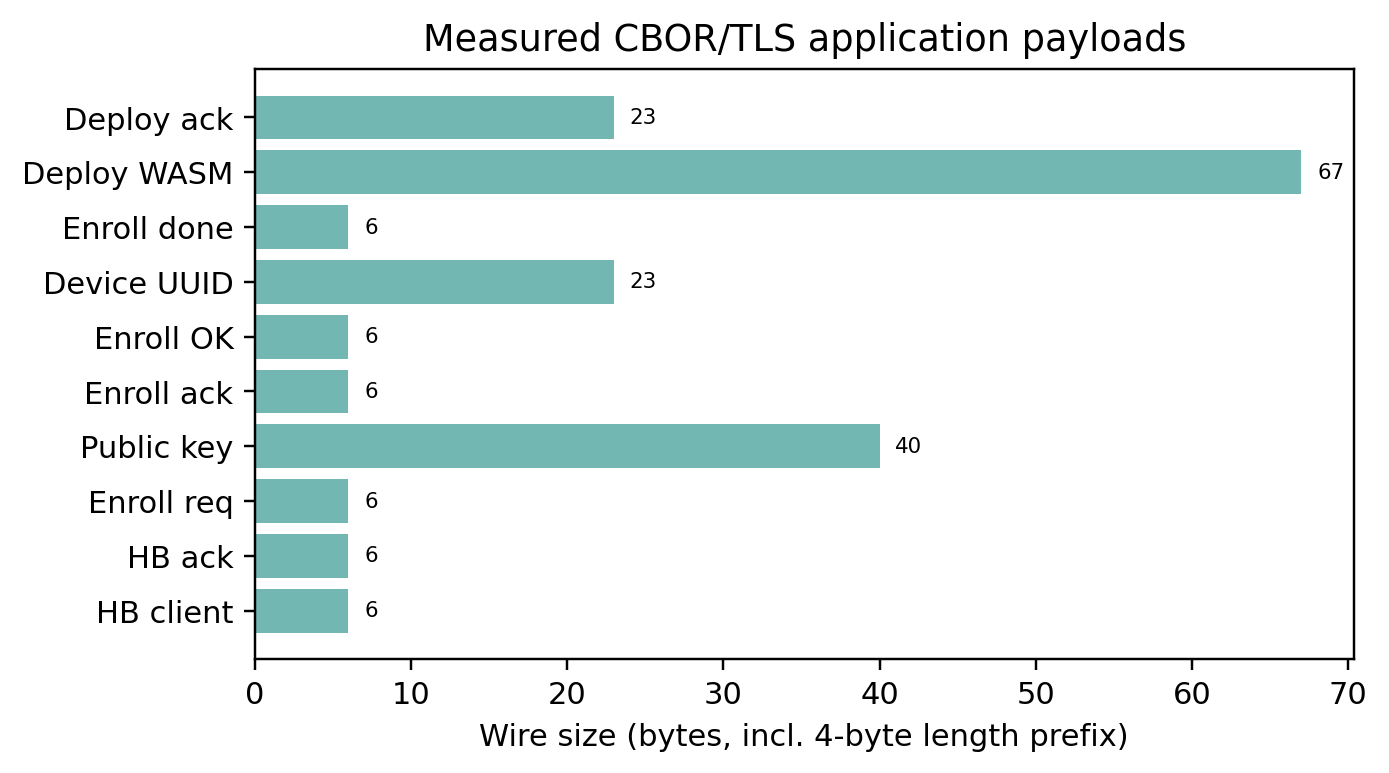
\includegraphics[width=\columnwidth]{figures/wire_sizes_bar.png}
\caption{Application-layer wire sizes (4-byte length prefix + CBOR) for representative protocol messages.}%
\label{fig:wire-sizes}
\end{figure}

\subsubsection{Edge footprint}
\begingroup
\color{red}
The evaluated Zephyr/WAMR/TLS/CBOR firmware fits the STM32F746NG internal-memory budget: the flash-resident \texttt{zephyr.bin} image is 406{,}568~B ($\approx$397~KiB), corresponding to text plus initialized data, and the static RAM allocation is 270{,}238~B ($\approx$264~KiB), corresponding to data (9{,}384~B) plus BSS (260{,}854~B).\footnote{The \texttt{zephyr.elf} file is 8{,}095{,}176~B (7.72~MiB), but only because it carries ELF metadata and debug symbols for the Renode \texttt{sysbus LoadELF} workflow; it is not the image written to device flash.} The benchmark WASM module remains 33~B. The architectural point supported by these measurements is therefore that embedded endpoints run no kubelet, container runtime, or Linux userspace while retaining an embedded-class memory footprint.
\endgroup


\subsubsection{Concurrent devices}\label{sec:concurrent-devices}
\begingroup
\color{red}
The trials above repeat one device through the full workflow, which measures the
workflow but says nothing about concurrency. A separate pass therefore attaches three
emulated STM32F746G devices at the same time. Each device carries its own enrollment
key, its own link-layer identity and its own DHCP lease, so the gateway, the control
plane and the network segment can all tell them apart; the identity a device presents
during enrollment is the one recorded in its Device resource.

All three attach and stay attached. The gateway runtime view lists three distinct
sessions, each with a heartbeat fresher than the 25~s firmware emission interval,
and the three Device resources independently reach \texttt{phase}\,=\,\texttt{Connected}
with their own liveness evidence. A single Application targeting all three devices
converges to \texttt{Running} on each of them: the gateway dispatches three separate
\texttt{DeployApplication} messages, one per session, and receives three successful
deployment acknowledgments. Because a deployment command travels only over the session
that belongs to its target device, three acknowledged deployments are direct evidence
of three independent southbound channels rather than of one channel reused.

Three devices on a single emulation host exercise session multiplexing, per-device
identity binding and per-device dispatch, establishing concurrency at the mechanism
level; Section~\ref{sec:discussion} states what this does not characterize.
\endgroup

\subsubsection{Control-plane resources}
Figure~\ref{fig:pod-resources} reports mean Kubernetes pod usage ($n{=}5$ samples, one TLS-connected device, sampled while the trial campaign was running). {\color{red}The metric is the container working set reported by \texttt{metrics-server}, cross-checked against cgroup~v2 \texttt{memory.current} and the anonymous resident set in \texttt{memory.stat}, which agree with it to within a few hundred kilobytes.} The gateway averaged 3.0~millicores CPU and 4.4~MiB RAM (\texttt{memory.current} 5.60~MB, anonymous 3.82~MB), the API server averaged 169.2~millicores and 33.4~MiB under campaign load (\texttt{memory.current} 32.3--33.0~MB), and the application controller averaged 38.4~millicores and 12.0~MiB (\texttt{memory.current} 13.3~MB). %Removed (minore): Registering 50 synthetic boards through the gateway HTTP registry left gateway resident memory unchanged (\texttt{memory.current} identical before and after), indicating lightweight per-device mediation state at the fog layer.
\revD{Registering 50 synthetic boards through the gateway HTTP registry left gateway
resident memory unchanged. This bounds the cost of registry state only: the boards are
\texttt{Device} entries rather than TLS-connected sessions, so the observation says nothing
about the per-session cost that would dominate a real fleet.}

\begin{figure}[pos=t]
\centering
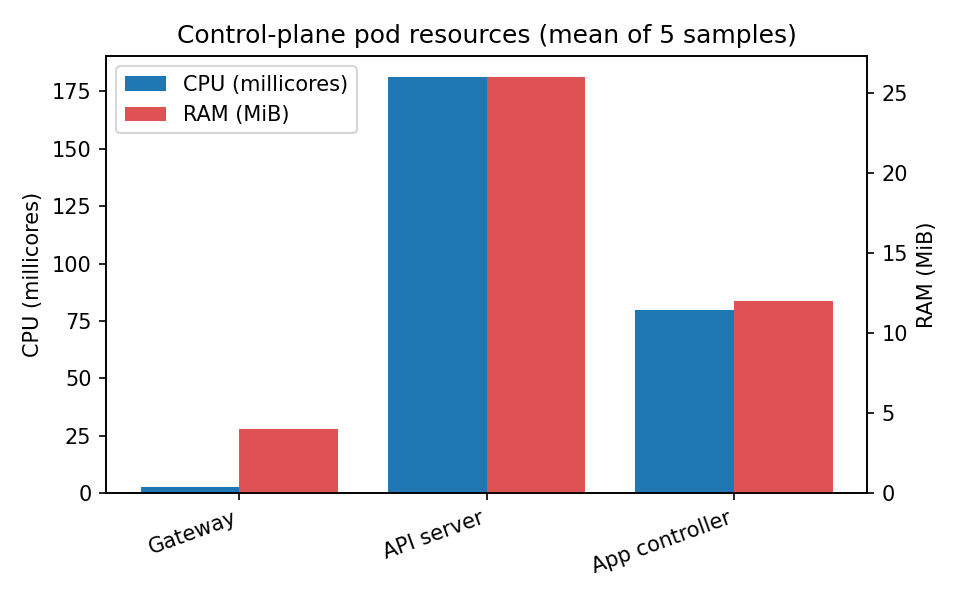
\includegraphics[width=\columnwidth]{figures/pod_resources_bar.png}
\caption{Mean CPU (millicores) and RAM (MiB) for control-plane pods during the sustainability measurement pass.}%
\label{fig:pod-resources}
\end{figure}

\begingroup
\color{blue}
\subsubsection{Computational energy instrumentation \revC{(measured CPU-time; derived energy and carbon as illustrative proxies)}}\label{sec:energy-instrumentation}
Beyond control-plane pod resources, we instrument a representative WASM computational workload directly. A Kubernetes pod running the fuel-metered Wasmtime runtime (\texttt{wasmbed-wasm-runtime}) repeatedly creates an isolated instance and executes a bounded arithmetic-loop WASM function (summing $0$ to $N$), cycling 30~s idle and 30~s active phases. This instruments a control-plane/fog-layer WASM execution path as a computational-energy proxy; 
%it does not measure the Renode-emulated STM32F746G/Zephyr/WAMR device evaluated elsewhere in this paper, since the embedded target is not directly instrumentable for energy in the present testbed. 
The pod runs under Guaranteed QoS (\texttt{requests}\,=\,\texttt{limits}, 2 vCPU) to remove self-induced CFS-throttling variance observed at the original 1-vCPU limit (835/27{,}021 accounting periods throttled under load, a scheduling artifact of the container's own quota, not of co-located tenants).

Two independent signals are collected. First, cgroup CPU time (\texttt{cpu.stat} \texttt{usage\_usec}) is an exact kernel accounting figure, not an estimate: at $N{=}200{,}000$, across $n{=}39$ paired cycles, the pod consumed $29.9289\pm0.0189$~CPU-s during each 30~s active window versus $0.000116\pm0.000053$~CPU-s during each equal-length idle window (paired difference 95\% CI $[29.9230, 29.9354]$~s, excluding zero). Second, we deploy Kepler~\cite{kepler} as a DaemonSet and query \texttt{kepler\_container\_joules\_total\{mode="dynamic"\}} scoped to the probe pod's own \texttt{pod\_name} label, isolating it from co-located wasmbed pods in the same namespace. 
Because the host is a virtualized guest without exposed RAPL counters, Kepler's output is a regression-based power estimate rather than a direct hardware measurement; with that caveat, it shows a clear and physically plausible increase under load: it attributes no dynamic power to the pod during the idle windows and $3.952$~W during the active ones (Figure~\ref{fig:energy-idle-active}). {\color{red}The exactly-zero idle attribution is a property of the estimator, not a measurement of the pod drawing no power.} We therefore treat the exact cgroup CPU-time as the primary, reproducible quantity throughout, and the Kepler wattage as a secondary, model-based signal consistent with it.

\begin{figure}[pos=t]
\centering
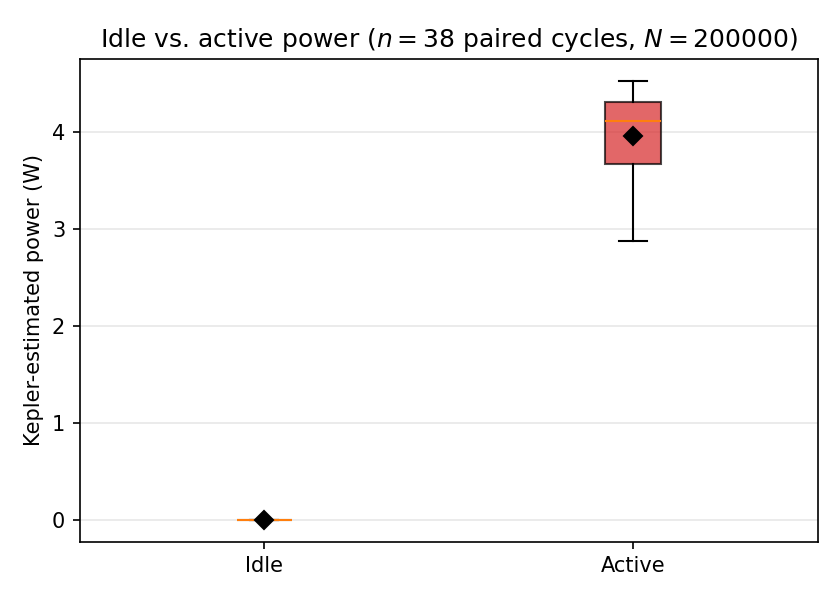
\includegraphics[width=\columnwidth]{figures/energy_idle_active_kepler.png}
\caption{Kepler-estimated power, idle vs.\ active phase ($n{=}38$ paired 30~s cycles with a power reading, $N{=}200{,}000$). Model-based estimate: this host exposes no RAPL counters.}%
\label{fig:energy-idle-active}
\end{figure}

Repeating the same idle/active protocol while varying the workload size $N \in \{50{,}000,\, 200{,}000,\, 1{,}000{,}000,\, 5{,}000{,}000\}$ ($n{\geq}10$ cycles per size) isolates CPU-time per WASM invocation from the fixed 30~s window: it grows from $95.9\,\mu$s at $N{=}50{,}000$ to $9.36$~ms at $N{=}5{,}000{,}000$. {\color{red}The two largest sizes exceed the MCU profile's default Wasmtime fuel budget of $5\times10^{6}$ units, which traps the call; they are measured with the budget raised (fuel metering still enabled), a change that alters no other aspect of the workload.} Plotted against an $O(N)$ reference line of slope~1 anchored at the smallest measured point, the four measurements track it closely across two orders of magnitude in $N$, consistent with the loop's linear time complexity rather than merely connecting four samples (Table~\ref{tab:workload-cpu-time}; 95\% CIs per point are narrower than the marker at this scale, $n{\geq}10$ cycles each).

\begin{table}[pos=t]
\centering
\caption{Workload size vs.\ measured CPU-time per invocation. \revC{CPU-s/call is exact kernel accounting; J/call is an \emph{illustrative range} spanning the two candidate per-vCPU full-load coefficients (4.72~W measured on the same part by a third party~\cite{epyc7313power}, 4.84~W from the manufacturer TDP~\cite{amd_epyc7313p}), and is read as an order of magnitude, not as a measurement.}}%
\label{tab:workload-cpu-time}
\footnotesize
\setlength{\tabcolsep}{3pt}
\begin{tabular}{rrrr}
\toprule
\textbf{$N$} & \textbf{$n$} & \textbf{CPU-s/call} & \revC{\textbf{J/call (illustrative)}} \\
\midrule
50{,}000 & 10 & $9.59\times10^{-5}$ & \revC{$4.5$--$4.6\times10^{-4}$} \\
200{,}000 & 39 & $3.77\times10^{-4}$ & \revC{$1.8\times10^{-3}$} \\
1{,}000{,}000 & 10 & $1.87\times10^{-3}$ & \revC{$8.8$--$9.0\times10^{-3}$} \\
5{,}000{,}000 & 10 & $9.36\times10^{-3}$ & \revC{$4.4$--$4.5\times10^{-2}$} \\
\bottomrule
\end{tabular}
\end{table}

Converting CPU-seconds into Joules requires a hardware-specific power coefficient, and this is the one step of the pipeline that is not measured on this platform. We therefore state its provenance explicitly. The primary reference is the manufacturer specification for the deployed processor, the AMD EPYC 7313P: 16 cores / 32 threads with a default TDP of 155~W and a configurable TDP of 155--180~W~\cite{amd_epyc7313p}, %Removed (minore): giving 4.84~W per vCPU at the default TDP.
giving 4.84~W per vCPU at the default TDP. \revD{The coefficient assumes that one vCPU
of the KVM guest of Table~\ref{tab:testbed} maps to one hardware thread of the host part,
which holds when the guest is not oversubscribed: the 32~vCPU guest matches the 32 threads
of the single socket. Under contention from other guests the effective per-vCPU power
would be lower than stated.} TDP is a thermal design limit rather than an instantaneous power draw, so it bounds rather than predicts consumption; as secondary corroboration, a third-party RAPL/\texttt{turbostat} measurement of the same single-socket part reports 35~W idle and 151~W full load across 32 threads~\cite{epyc7313power}, i.e.\ 1.09~W and 4.72~W per vCPU, within 3\% of the specification-derived value. Neither figure is a measurement of this workload on this hardware, and a platform-specific coefficient would come from a documented energy benchmark such as SPECpower\_ssj2008~\cite{specpower} or the per-family coefficient table of the Cloud Carbon Footprint project~\cite{ccf}. \revC{The conversion also rests on a deliberately simple model --- power proportional to allocated vCPU-time at full load --- which ignores the idle baseline, DVFS and turbo behaviour, shared uncore, memory and I/O power, and the known non-linearity of power against utilization. Each effect can move the result by tens of percent in either direction, which is why every derived figure below is given to at most two significant digits; removing the assumption requires re-anchoring the pipeline on a host exposing RAPL counters.}
Applying the Cloud Carbon Footprint average-wattage formula~\cite{ccf} to the measured utilization yields \revC{${\approx}119$}~J attributable to the active window above its idle baseline (\revC{${\approx}1.5$}~mJ per WASM invocation over ${\approx}$79{,}300 invocations per window). Carbon follows from that energy and a grid emission factor, and is reported here parametrically for the same reason: at an intensity $I$, the active window accounts for \revC{${\approx}33\,I$}~$\mu$gCO\textsubscript{2}eq with $I$ in gCO\textsubscript{2}eq/kWh. We take $I$ from the institutional source for Italy, the ISPRA national consumption-mix emission factor, 199.61~gCO\textsubscript{2}eq/kWh for 2025 (preliminary estimate)~\cite{ispra_settore_elettrico}, which puts the active window at \revC{${\approx}6.6$~mgCO\textsubscript{2}eq (of order $0.1$~$\mu$gCO\textsubscript{2}eq per invocation)}. Production- and consumption-mix factors differ and the choice must be stated with the value; the European Environment Agency indicator~\cite{eea_grid_intensity} provides the corresponding cross-country basis. 
%\revC{The measured claims of this subsection are therefore the CPU-time quantities alone; everything in Joules or grams of CO\textsubscript{2}eq is a proxy computed from them with an external coefficient, and no conclusion of this paper depends on its absolute value.}

\paragraph{Per-phase, per-pod CPU-time (control-plane trials).} %Removed (minore): As a minimal, additive instrumentation point layered on the trial harness behind Table~\ref{tab:quantitative-latency} (no change to gateway, controller, or reconciler logic), each
\revD{As an instrumentation point layered on the trial harness behind Table~\ref{tab:quantitative-latency}, leaving gateway, controller and reconciler logic unchanged, each} of the enrollment, heartbeat, and deployment stages is separately bracketed by a \texttt{cpu.stat} \texttt{usage\_usec} snapshot for the gateway, API-server, and application-controller pods, giving CPU-seconds consumed by each pod during exactly that stage's wall-clock window. %Removed (M8): The measurement runs against the full live stack: a Zephyr~3.5.0/WAMR firmware image for the emulated STM32F746G target, connected to the gateway over TLS through the Renode TAP bridge.
\revD{The measurement runs against the full live stack: a Zephyr~3.5.0/WAMR firmware
image for the emulated STM32F746G target, connected to the gateway over TLS through the
Renode TAP bridge. The two provisioning paths mentioned above are not alternatives here
but successive steps of the same trial. The board is first registered through the gateway's
auxiliary HTTP endpoint, which creates the \texttt{Device} resource and its expected
identity; the firmware then attaches over TLS and drives the same enrollment exchange as
the campaign of Table~\ref{tab:quantitative-latency}, so each record carries both a
registered board and a \texttt{Device} that reaches \texttt{phase}\,=\,\texttt{Connected}
with a fresh heartbeat. The difference from the main campaign is that registration is
performed explicitly rather than assumed from a pre-existing resource, which shifts a small
and constant amount of API-server work into the enrollment window; the stages themselves
are the same, and the two sets of latencies are not intended to be compared.} Table~\ref{tab:cpu-time-per-phase} reports a $n{=}5$-trial pass: all three stages succeed 5/5, with real, reproducible CPU-time per stage per pod, and the enrollment row covers the full protocol exchange (TLS handshake, CBOR EnrollmentRequest/PublicKey/DeviceUuid, gateway-side connection established) up to the Device CRD reaching \texttt{status.phase}\,=\,\texttt{Connected}.

Given $n{=}5$, this table demonstrates the instrumentation working end-to-end on real infrastructure rather than providing a statistically powered per-stage estimate; a $n{=}100$ run aligned with Table~\ref{tab:quantitative-latency} is future work.

\begin{table}[pos=t]
\centering
%Removed (M8): \caption{CPU-seconds per phase per pod ($n{=}5$ trials, \revC{provisioned through the auxiliary HTTP registry endpoint}; all three stages succeeded 5/5). Exact cgroup \texttt{cpu.stat}, not an estimate.}%
\caption{CPU-seconds per phase per pod ($n{=}5$ trials, \revD{board registered through the gateway HTTP endpoint and then enrolled over TLS}; all three stages succeeded 5/5). Exact cgroup \texttt{cpu.stat}, not an estimate.}%
\label{tab:cpu-time-per-phase}
\footnotesize
\setlength{\tabcolsep}{2pt}
\resizebox{\columnwidth}{!}{%
\begin{tabular}{llrrrr}
\toprule
%Removed (M8): colonne p95 e IC-t sostituite da min--max e bootstrap; valori originali:
%\textbf{Stage} & \textbf{Pod} & \textbf{Mean} & \textbf{Median} & \textbf{p95} & \textbf{95\% CI of mean} \\
%Enrollment & gateway & 0.000350 & 0.000326 & 0.000503 & [0.000239, 0.000462] \\
%Enrollment & api-server & 0.143510 & 0.083265 & 0.384413 & [$-$0.023697, 0.310717] \\
%Enrollment & app-controller & 0.036625 & 0.035557 & 0.045817 & [0.029140, 0.044109] \\
%Heartbeat & gateway & 0.000413 & 0.000390 & 0.000684 & [0.000206, 0.000620] \\
%Heartbeat & api-server & 0.020483 & 0.000000 & 0.102417 & [$-$0.036379, 0.077345] \\
%Heartbeat & app-controller & 0.010088 & 0.010080 & 0.010956 & [0.009043, 0.011133] \\
%Deployment & gateway & 0.006338 & 0.006521 & 0.008674 & [0.003693, 0.008984] \\
%Deployment & api-server & 0.564172 & 0.465255 & 0.823915 & [0.280249, 0.848096] \\
%Deployment & app-controller & 0.057557 & 0.027365 & 0.111654 & [$-$0.002620, 0.117734] \\
\textbf{Stage} & \textbf{Pod} & \textbf{Mean} & \textbf{Median} & \revD{\textbf{Min--max}} & \revD{\textbf{95\% CI (bootstrap)}} \\
\midrule
Enrollment & gateway & 0.000350 & 0.000326 & \revD{0.000266--0.000503} & \revD{[0.000291, 0.000432]} \\
Enrollment & api-server & 0.143510 & 0.083265 & \revD{0.080665--0.384413} & \revD{[0.082006, 0.264079]} \\
Enrollment & app-controller & 0.036625 & 0.035557 & \revD{0.030778--0.045817} & \revD{[0.032261, 0.041684]} \\
Heartbeat & gateway & 0.000413 & 0.000390 & \revD{0.000227--0.000684} & \revD{[0.000292, 0.000563]} \\
Heartbeat & api-server & 0.020483 & 0.000000 & \revD{0.000000--0.102417} & \revD{[0.000000, 0.061450]} \\
Heartbeat & app-controller & 0.010088 & 0.010080 & \revD{0.009197--0.010956} & \revD{[0.009415, 0.010760]} \\
Deployment & gateway & 0.006338 & 0.006521 & \revD{0.003787--0.008674} & \revD{[0.004659, 0.008018]} \\
Deployment & api-server & 0.564172 & 0.465255 & \revD{0.307216--0.823915} & \revD{[0.390794, 0.739244]} \\
Deployment & app-controller & 0.057557 & 0.027365 & \revD{0.019152--0.111654} & \revD{[0.021213, 0.093901]} \\
\bottomrule
\end{tabular}%
}
\end{table}
\endgroup

\subsubsection{Architectural comparison}
Table~\ref{tab:arch-compare} contrasts gateway-mediated WASM orchestration with treating each constrained device as a Kubernetes worker. % Removed: Edge Kubernetes deployments commonly require tens to hundreds of MiB of resident memory per worker for kubelet and container runtime before user workloads~\cite{kubernetes}.
{\color{red}Edge Kubernetes deployments require a Linux-capable node with a kubelet, container runtime, and supporting operating-system services before user workloads, whereas the evaluated endpoint keeps those cluster agents off the device.} %Removed (M6): Our design concentrates orchestration in a shared gateway (under 5~MiB measured) while keeping cluster agents off the device.
\revD{Our design concentrates orchestration in a shared gateway (under 5~MiB measured)
while keeping cluster agents off the device. The comparison is a qualitative contrast of
architectural models, not a measured benchmark: only the right-hand column is instrumented
here, and establishing the left-hand one would require running the same WASM workload on a
Linux single-board node with a cluster agent. The pod measurements also locate the real
cost differently from the intuition the table invites. Mediation is cheap---the gateway
averages 3.0~millicores---while the API server averages 169.2~millicores, so the
control plane, not the fog layer, dominates control-plane CPU at this scale. Whether
gateway mediation remains cheaper than per-device agents therefore depends on fleet size
through a break-even this evaluation does not determine.}

\begin{table}[pos=t]
\centering
%Removed (M6): \caption{Orchestration model comparison.}%
\caption{\revD{Qualitative contrast of orchestration models. Only the gateway-mediated column is measured in this work.}}%
\label{tab:arch-compare}
\footnotesize
\setlength{\tabcolsep}{3pt}
\begin{tabular}{p{0.22\linewidth} p{0.34\linewidth} p{0.34\linewidth}}
\toprule
\textbf{Aspect} & \textbf{Device as K8s worker} & \textbf{Gateway-mediated WASM edge} \\
\midrule
Edge runtime & kubelet + container runtime + OS & Zephyr + WAMR ({\color{red}397~KiB flash, 264~KiB RAM}) \\
% Removed: Edge cluster agent RAM & 100--350~MiB per node (literature) & none on device \\
{\color{red}Edge cluster agent footprint} & {\color{red}kubelet + container runtime + OS services required} & none on device \\
% Removed: Steady control traffic & CRI/container probes & 1728~B/h per device \\
{\color{red}Steady heartbeat traffic} & CRI/container probes & {\color{red}1728~B/h per device (application layer)} \\
Fog mediation RAM & per-node agent & ${<}5$~MiB shared gateway \\
\bottomrule
\end{tabular}
\end{table}
